\documentclass{cernatsnote}
\usepackage[colorinlistoftodos]{todonotes}
\usepackage{placeins}

\usepackage{booktabs}
\usepackage{enumitem}
\usepackage{hyperref}
\usepackage[parfill]{parskip}
\usepackage{siunitx}
\usepackage{stfloats}

\title{Technical design of the Bmboot monitor}
\author{
	Martin Cejp \; \\		
	CERN, CH-1211 Geneva, Switzerland
}
\email{martin.cejp@cern.ch}
\date{Version XX, \today}
\documentlabel{\href{https://edms.cern.ch/document/3028102}{EDMS 3028102}}
\keywords{{\tt real-time control, bare-metal, Cortex-A53, AArch64}}

\begin{document}
\maketitle

\begin{abstract}
This document describes the detailed design of Bmboot, a bare-metal privileged monitor for the Zynq UltraScale+ MPSoC, which incorporates a Cortex-A53 CPU, itself an implementation of the ARMv8-A architecture.

This document accompanies the user-facing Bmboot documentation available at \url{https://bmboot.docs.cern.ch}. It is primarily aimed at those needing to maintain, extend, or debug Bmboot.
\end{abstract}
\\ \\ \\ 

\begingroup
\color{black}
\tableofcontents
\endgroup

\pagebreak

\section{The need for a bare-metal monitor}

The FGC4 platform has some ambitious goals: in particular, a desired iteration rate of \qty{100}{\kHz} with non-trivial control algorithms. When the execution time budget is just \qty{10}{\us} per iteration, some traditional software engineering practices must be revised. As reported in~\cite{zielinski:task-isolation}, a Linux system, even when carefully tuned for real-time performance, does not provide the necessary predictability of execution timing.

It was therefore decided to dedicate some cores of the Cortex-A53 CPU to execute a bare-metal real-time loop. This, indeed, gives the developer full control and a high-degree of performance predictability. However, it comes at a cost; a~number of features and protections normally provided by the operating system (OS) have to be given up:

\begin{itemize}
    \item There is no mechanism to load, start and stop programs. The developer takes full responsibility of preparing the program image, loading it in memory, and pointing the CPU to its first instruction.
    \item In absence of memory protection, the execution environment becomes a fragile house of cards. An erroneous memory access can crash not only the faulty program, but the entire CPU.
    \item Operating systems provide convenient abstractions for input and output, which can be, for example, transparently re-routed over the network. Bare metal code only has access to low-level hardware peripherals such as GPIO, UART or SPI.
    \item Without virtual memory, greater care must be taken in regards to memory management. Repeated allocation and de-allocation can leave the memory fragmented, limiting the size of a contiguous block that can be allocated, regardless of the total amount of free memory.
\end{itemize}

Although most of these issues can be overcome, they add enough friction to slow down development and increase the cost of testing. The lack of solid protection mechanisms can also pose a risk in an operational deployment.

\clearpage
\section{Hardware features enabling monitor implementation}

The target platform is the Zynq UltraScale+ MPSoC, which incorporates a Cortex-A53 CPU with 2 or 4 cores, depending on the specific part. This CPU, in turn, implements the 64-bit ARMv8-A architecture. Combined, these ``architectural layers'' provide a set of features that make it feasible to implement a monitor program substituting some of the features and protections of a traditional operating system.

\subsection{CPU core control}

When the CPU is powered on, all cores except one (CPU0) are in a \textit{power-on reset} state. They remain in reset until the operating system clears the corresponding bit in a machine register which controls this state.

By manipulating the \textit{device tree}, the OS can be told to ignore certain CPU cores. In that case, they would remain in reset indefinitely. However, the same mechanism used by the OS to start a core can also be used by user code (provided that some default protections in the OS are lifted). This way, a developer can start their own bare-metal program on these additional cores.

It would seem natural that the same machine register could be used to re-assert the reset state and prepare the CPU core to run a new application. However, this is not the case. Attempting to stop a core which is executing code is unpredictable and often leads to a lock-up of the entire system. \cite{zynqmp-trm}

\subsubsection{Power State Coordination Interface}

The ARM firmware implements Power State Coordination Interface (PSCI), which is a standard interface that allows an OS to start and stop CPU cores at will. The Linux kernel implements this interface, but it is not exposed to user-mode programs.

Paradoxically, user-mode code must resort to lower-level means of controlling core reset state, which is through the \texttt{RST\_FPD\_APU} register \cite{zynqmp-registers} and the \texttt{RVBARADDR} family of registers \cite{zynqmp-trm}.

\subsection{Exception levels}

% Note: capitalized as "Exception level" as per ARM docs

The CPU architecture distinguishes different levels of privilege of the software being executed. Generally speaking, more privileged levels have authority over less privileged levels. Additionally, the CPU provides mechanisms to prevent less privileged code from interfering with the execution of more privileged code. This is implemented by means of \textit{Exception levels} (EL). Four exception levels are defined, EL0 through EL3. By convention, they correspond to the different layers of software indicated in Table~\ref{tab:exception-levels}.

\begin{table}[h]
  \centering
  \begin{tabular}{ll}\toprule
  \textbf{EL} & \textbf{Conventional usage}\\\midrule
    EL3 & Secure monitor \\
    EL2 & Hypervisor \\
    EL1 & Operating system \\
    EL0 & User application (least privileged) \\\bottomrule
  \end{tabular}

  \caption{Assignment of Exception levels.}
  \label{tab:exception-levels}
\end{table}

The usage intended by the designers is reflected in the fact that not all features are available at all levels. Therefore, an attempt to implement a different software stack-up may run into limitations. To give a concrete example, interrupts cannot be delivered to code at EL0; a handler must be implemented on EL1 or above.

\subsubsection{System calls \label{syscall-instructions}}

The architecture provides dedicated instructions to invoke services provided by higher ELs. Executing one of these instructions triggers an exception handler on the corresponding EL. This handler can then process the request and perform the corresponding action.

The instructions are:

\begin{itemize}
    \item \texttt{SVC} (Supervisor Call) to call into EL1
    \item \texttt{HVC} (Hypervisor Call) to call into EL2
    \item \texttt{SMC} (Secure Monitor Call) to call into EL3
\end{itemize}
	\clearpage
\section{Bmboot architecture}

Figure~\ref{fig:components} illustrates a typical application, consisting of a Linux counterpart and a bare-metal counterpart. The core or cores running Linux (collectively the \textit{Linux Realm}) take the role of managing the \textit{executors} -- cores dedicated to executing bare-metal programs.

Bmboot provides a number of key components enabling this workflow, described in the following sections.

\begin{figure}[h]
  \centering
  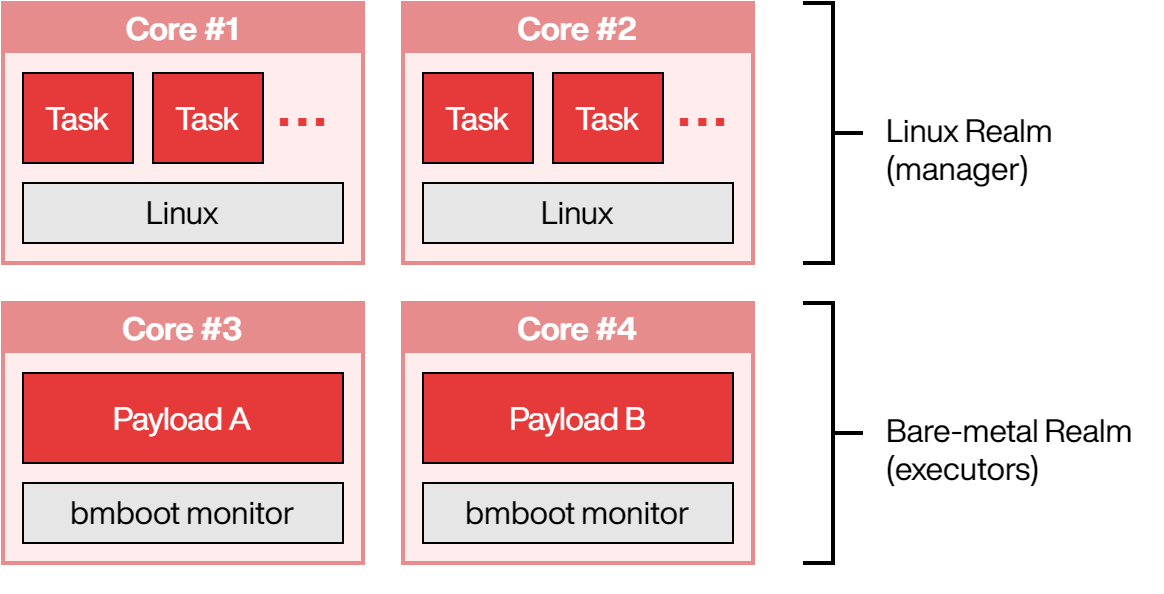
\includegraphics[width=0.8\textwidth]{images/realms-simplified.png}
  \caption{Components in a complete system using Bmboot \label{fig:components}}
\end{figure}

\subsection{Core components}

\subsubsection{Payload}

Payload is the user's real-time application. It executes under the supervision of the monitor and can make use of APIs provided by the monitor. To function properly, the payload must respect the execution environment and must be compiled in a prescribed way.

\subsubsection{Bare-metal monitor}

The bare-metal monitor executes on the same core as the payload. It starts the payload and provides services to it via an API. The monitor can be called upon to interrupt the execution of the payload, but otherwise does not interfere with it during normal execution.

\subsubsection{Payload runtime library}

The monitor's API is exposed to the payload through a small library of functions that is linked into the payload. Internally, it makes use of a mechanism similar to the \textit{syscall} in a traditional OS to change the execution context from user application into the monitor.

\subsubsection{Manager library and command-line tools}

On the Linux side, an application can control the life-cycle of the bare-metal application through a library that is provided. Alternatively, if the bare-metal application is able to function without a Linux counterpart, it can be managed using a provided command-line tool (\texttt{bmctl}).

\subsection{Memory organization and management}

\begin{figure}[h]
  \centering
  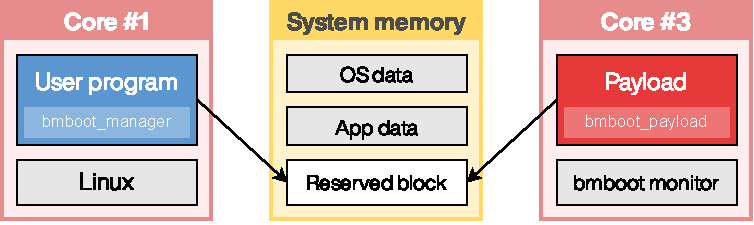
\includegraphics[width=0.9\textwidth]{images/memory-arch.pdf}
  \caption{Each executor has a dedicated block of memory for communication with the manager}
\end{figure}

The design is based on the assumption of a cache-coherent memory system. Regions of physical memory are marked as ``reserved'' in the system device tree; this excludes them from being managed by Linux and makes them safe to use by bare-metal code.

The need for manual address allocation and modification of the device tree in an inconvenience, but there is a number of reasons for it:

\begin{itemize}
    \item Monitor and payload binaries are non-relocatable -- the run-time layout of the physical memory must already be known at the time when these binaries are built.
    \item The alternative to modifying the device tree would be to have a kernel driver allocate some contiguous physical memory. Maintaining a kernel driver is not a trivial task and we prefer to avoid it.
    \item A predictable memory layout reduces the number of ``moving parts'' and simplifies debugging.
\end{itemize}

Each Bmboot-controlled CPU core requires its own instances of the following memory regions:

\begin{itemize}
    \item monitor binary (all-inclusive: code, static variables, stack, heap)
    \item an \textit{IPC Block} between the monitor and manager
    \item payload binary
\end{itemize}

It is expected that a typical user application will additionally dedicate some memory to exchange application-specific data.

Note: No memory protection is implemented at the time of writing.

\subsubsection*{FGC4 specifics}

\begin{enumerate}
    \item To ease the task of memory assignment, FGC4 includes a utility called \texttt{mmtool} to generate C/C++ headers and linker scripts with addresses of the various memory regions.
    \item A relatively large chunk of physical memory is dedicated to a so-called \textit{pool}. When the application starts, blocks are allocated from the pool for various purposes like log buffers.
\end{enumerate}

% To review: https://github.com/ceph/dpdk/blob/master/lib/librte_eal/linuxapp/eal/eal_memory.c

\subsubsection{Cache concerns during application startup}

A fundamental assumption in the design of Bmboot is that the memory system is cache-coherent. That is, when one CPU core writes to a physical memory location, other cores subsequently reading from the same location will observe the new value. Moreover, the observed order of memory operations is the same for all cores.

The CPU provides hardware support for cache coherence, by means of the \textit{Snoop Control Unit} (SCU). However, there are prerequisites that must be satisfied: the memory must be configured as cacheable by all participants, since uncached accesses are not broadcast to other cores.
The insidious thing is that with incorrect setup, the programs might still execute correctly due to luck -- until a small change is made and suddenly they don't.

When the Bmboot monitor is started for the first time, the core is in its default reset configuration, which disables all caches. One of the first steps is to enable caching, so that future memory operations are coherent. Until that point has been reached, care must be taken to manually flush each range of memory modified by one core and read by another.

\subsection{Executor state machine \label{subsec:executor-fsm}}

When a CPU core is put under the control of Bmboot, it becomes an \textit{executor domain}\footnote{The terminology was inspired by the Xen hypervisor, where a \textit{domain} refers to a virtual machine. In Xen, domains can be created at will, while in Bmboot, there is a fixed number of domains corresponding one-to-one to the available CPU cores.}, or simply \textit{executor}. The lifecycle of an executor is controlled by the monitor, based on commands from the manager, following the state machine depicted in Figure~\ref{fig:state-machine}.

\begin{figure}[h]
  \centering
  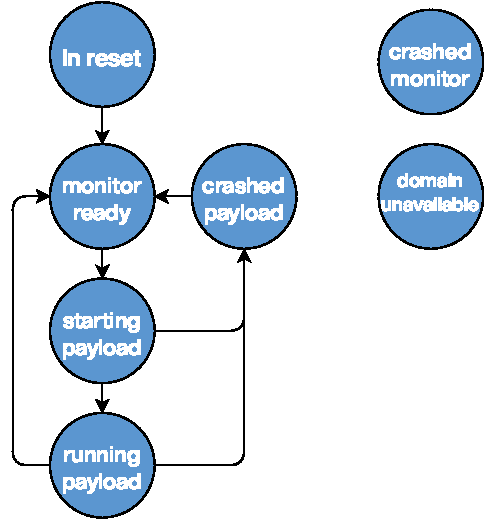
\includegraphics[width=0.55\textwidth]{images/executor-fsm.pdf}
  \caption{Executor domain state machine \label{fig:state-machine}}
\end{figure}

At the beginning, an executor core must be in power-on reset. Otherwise, the manager will determine that there is already other code executing (perhaps the core is being used by Linux) and will deem the domain \textit{unavailable}.

It is important to note that no persistent state is being kept on the manager side; every time a new access to a domain is initiated (whether through the \texttt{bmctl} utility or the \texttt{IDomain::open} API function), it is necessary to determine whether the domain is under the control of Bmboot or not. This process is described by Figure~\ref{fig:state-determination}: if the CPU core in question is already executing code, a specific signature value, placed at a fixed memory address, is used to distinguish between a core under Bmboot control and a core executing other code. This is a heuristic approach; a challenge--response mechanism would provide more confidence. However, this would conflict with the design requirement to not interrupt a running payload unless it needs to be terminated.

\begin{figure}[h]
  \centering
  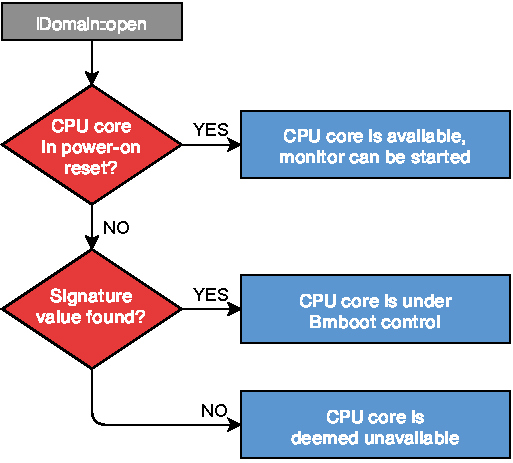
\includegraphics[width=0.65\textwidth]{images/state-determination.pdf}
  \caption{Executor domain state determination flow chart \label{fig:state-determination}}
\end{figure}

\subsection{Communication between manager and monitor}

The manager issues commands to the monitor through the IPC block. Commands are only processed when the domain is in \texttt{monitor ready} state. Only one command is currently implemented, \texttt{start payload}.

A different approach is necessary when the manager needs to terminate a running payload, since the monitor is not active in this state, and commands are therefore not being executed. For this purpose, an intrusive mechanism called \textit{inter-processor interrupt} (IPI), described further in subsection~\ref{ssec:ipi}, is used.

\subsection{Payload execution environment}

Bmboot payloads execute in an environment with many similarities to other embedded platforms without operating system.

It is possible to use many functions from the C standard library, and even some functions from POSIX including:

\begin{itemize}
    \item math functions
    \item string functions
    \item memory allocation
    % \item \texttt{usleep}
    \item standard output (\texttt{printf} et al.)
\end{itemize}

Many classes from the C++ Standard Template Library are also safe to use:

\begin{itemize}
    \item containers (array, map, vector)
    \item strings
    \item utility classes, such \texttt{std::optional}
    \item exceptions
\end{itemize}

On the other hand, the following facilities are \textit{not} available:

\begin{itemize}
    \item file I/O
    \item standard input
    \item threads
    \item signals
    \item networking
\end{itemize}

The technical explanation is that only those parts of the library that do not depend on \textit{syscalls} can be safely used. As there is no operating system, the majority of syscalls are not available, and this extends to any functionality relying on them. Some syscalls are available, either by emulating them inside the payload runtime (\texttt{\_sbrk}) or by calling into the monitor (\texttt{\_write}).

Caution must be exercised when using dynamic memory allocation, especially indirectly (e.g., \texttt{std::vector}). As there is no virtual memory, the environment is particularly prone to memory fragmentation, which over time limits the maximum size of a contiguous block that can be allocated, regardless of the total free memory.

Payloads execute in a flat memory space. The particular load address will depend on which CPU is executing the payload. By default, the program will be able to access all of physical memory. This includes parts of the address space which do not correspond to valid memory and which can destabilize the system if an access is attempted.
	\clearpage
\section{CPU configuration and startup procedures}

This section details the configuration of the CPU cores and the exact steps taken when starting up.

\subsection{Monitor startup}

The first part of the procedure is carried out by the manager.

\begin{enumerate}
    \item The appropriate monitor binary is selected based on the CPU core number (recall that bare-metal code is not relocatable and each core uses a different memory range)
    \item The binary is copied to the corresponding memory location
    \item The Bmboot signature value is written (see subsection~\ref{subsec:executor-fsm})
    \item The primary memory structure for manager-executor communication (IPC block) is initialized
    \item All memory regions affected in the previous steps are flushed to main memory
    \item The \texttt{RVBARADDR} registers are set to the starting code address
    \item The \texttt{RST\_FPD\_APU} register is used to clear the power-on reset state of the CPU core and begin code execution in EL3
    \item The monitor initializes and sets its reported state (\texttt{ipc\_block.executor\_to\_manager. state}) to \texttt{monitor\_ready}. This concludes the procedure.
\end{enumerate}

\subsection{Payload startup}

Once the monitor is ready, the manager can request to start a payload. The payload expects to execute in EL1 from the start, which is reflected in the following procedure, derived from~\cite{arm-baremetal} and implemented in \textit{monitor\_asm.S}.

\begin{table}[h]
  \centering
  \begin{tabular}{rlrp{9cm}}\toprule
  \textbf{Bit(s)} & \textbf{Name} & \textbf{Assigned value} & \textbf{Explanation}\\\midrule
    0 & NS & \textbf{1} & EL1 is in Non-secure state. It might not matter much, but it is what the Xilinx SDK expects. \\
    1 & IRQ & \textbf{0} & IRQs are \textit{not} intercepted by EL3. While executing in EL3, IRQs will be ignored because we keep the \texttt{I} flag set. When executing on a lower level, they are routed correspondingly (in our case to EL1). \\
    2 & FIQ & \textbf{1} & FIQs are always taken to EL3. \\
    3 & EA & \textbf{1} & External Aborts and SErrors are taken to EL3. \\
    7 & SMD & \textbf{0} & \texttt{SMC} instruction is enabled. \\
    8 & HCE & \textbf{0} & \texttt{HVC} instruction is disabled. \\
    9 & SIF & \textbf{0} & Allow execution of code from Non-secure memory even in Secure mode. \\
    10 & RW & \textbf{1} & EL2 is AArch64 and lower levels are determined by EL2 configuration. \\\bottomrule
  \end{tabular}

  \caption{Bit assignment in the \texttt{SCR\_EL3} register. The register contains additional bits which we consider uninteresting and they are set to zero.}
  \label{tab:scr-el3}
\end{table}

\begin{enumerate}
    \item \texttt{SCR\_EL3} (Secure Configuration Register), which controls several aspects of the relationship between EL3 and EL1, is updated with the values in Table~\ref{tab:scr-el3}.\footnote{This register is initially configured in \textit{boot.S} and in principle, it could be programmed with the necessary values from the beginning.}
    \item \texttt{HCR\_EL2} is set to all-zero, save for bit 31 (\texttt{RW}) to indicate AArch64 mode for EL1. \texttt{HCR\_EL2} can be thought of as the EL2 analog of \texttt{SCR\_EL3}, in that it controls the relationship to lower ELs.
    \item \texttt{SCTLR\_EL1} is set to \texttt{0x30C50838}, which is the default reset value. Payload start-up code will reconfigure this register once more.
    \item \texttt{SPSR\_EL3} (Saved Program Status Register) is set to \texttt{0b00101}, indicating \textit{EL1 with dedicated stack pointer} (EL1h)
    \item \texttt{ELR\_EL3} (Exception Link Register) is set to the payload's entry point address
    \item An \texttt{ERET} instruction is executed to perform the transition to EL1, jumping to the address specified in \texttt{ELR\_EL3}.
\end{enumerate}

After this, the payload begins executing. The very first code executed is that in \textit{asm\_vectors.S}, but the main body of initialization can be found in \textit{boot.S} and subsequently \textit{xil-ctr0.S}, before finally branching to the user-defined \texttt{main} function.


\subsection{Architectural timer}

Each core of the Cortex-A53 CPU contains a private timer/counter. The pitfall lies in the fact that frequency is configurable at system design time (in Vivado).

\begin{itemize}
    \item When generating the XSA file, psu\_init.c will contain initialization of a control register called \texttt{TIMESTAMP\_REF\_CTRL}. The initialization value is presumably derived from the user-specified desired timer frequency and from the system clocking information (reference freq. coming from the crystal, or something like that)
    \item When generating the BSP in Vitis, \textit{a53/xparameters.h} defines the constant \\ \texttt{XPAR\_PSU\_CORTEXA53\_0\_TIMESTAMP\_CLK\_FREQ}, indicating the frequency in Hz
    \item BSP default \textit{boot.S} places the value of this constant into \texttt{CNTFRQ\_EL0}, so that software can always read it from there instead of having to derive it based on \texttt{TIMESTAMP\_REF\_CTRL}
\end{itemize}

Note: \texttt{TIMESTAMP\_REF\_CTRL} is SoC-level, but the \texttt{CNTFRQ\_EL0} register is private to each core.

This is not really a problem for true bare-metal applications which are fixed to a specific board, but when compiling the Bmboot monitor, it is undesirable to fix the timer frequency inside the compiled code. For detecting it at runtime, we have a number of options:

\begin{enumerate}[label=(\alph*)]
    \item Try to reconstruct the frequency on bare metal by reading \texttt{TIMESTAMP\_REF\_CTRL}
    \item Extract the value on Linux (Linux knows for sure: \texttt{arch\_timer\_rate} in \textit{arm\_arch\_timer.c}; but is there any way to extract this value?) and pass it to the monitor when starting it. The monitor will then put this into \texttt{CNTFRQ\_EL0}.
    \item Require the user to provide a ``board specification file'' at runtime where Bmctl can read the frequency and pass it on as in option 2. This could be also used to specify the CPU indexes.
\end{enumerate}

Examples:

\begin{itemize}
    \item \url{https://github.com/Xilinx/embeddedsw/blob/master/lib/sw\_apps/zynqmp\_fsbl/misc/zcu102/psu\_init.c}
    \item \url{https://github.com/Xilinx/embeddedsw/blob/master/lib/sw\_apps/zynqmp\_fsbl/misc/zcu102/a53/xparameters.h}
\end{itemize}
	\clearpage
\newcommand{\ELRELn}{\texttt{ELR\_EL\textit{n}}}
\newcommand{\SPSRELn}{\texttt{SPSR\_EL\textit{n}}}

\section{Exceptions and interrupts}

AArch64 CPUs implement 4 types of exceptions:

\begin{enumerate}
  \item synchronous exception
  \item interrupt request (IRQ)
  \item fast interrupt request (FIQ)
  \item system error (SError)
\end{enumerate}

Generally speaking, a synchronous exception is triggered when the program tries to perform either an invalid,
or somehow ``special'' operation.
In the context of Bmboot, the former case would be an error in the payload, such as invalid memory access,
and the latter could be an SMC. (Secure Monitor Call -- see subsection~\ref{syscall-instructions})

IRQ and FIQ are triggered by external sources -- mostly hardware peripherals.
One important exception is the inter-processor interrupt (IPI), which is sent from one CPU core to another.
In Bmboot this is used to abort the running payload and return control to the monitor.
This would be normally done if the payload crashes or hangs, or if the application needs to load another payload.

An exception can be \textit{taken to} either the current or higher EL, and the handler can return to the same or lower EL. An exception being taken to a higher EL means that the CPU core switches to this EL before the corresponding exception handler begins executing. Under no circumstances do exceptions cause a transition to a lower EL (see also \cite{arm-arm}, chapter D1.10). Whenever in doubt, remember that higher ELs are considered privileged and taking an exception to a \textit{lower} EL would leak register contents, potentially revealing sensitive information to an unprivileged application.

\subsection{Relevant exception sources}

See Table~\ref{tab:int-sources}.

\begin{table}[b]
  \centering
  \begin{tabular}{lccp{6.2cm}}\toprule
  \textbf{Exception source} & \textbf{Exc. type} & \textbf{Handled in} & \textbf{Comment} \\\midrule
  EL1 call to EL3 (\texttt{SMC}) & Sync & EL3 & Used to implement monitor services \\
  Fault in monitor & Sync & EL3 & Fatal error in the monitor \\
  Fault in payload & Sync & EL1 & Caught in EL1, then escalated to EL3 via \texttt{SMC} \\
  External GPIO & IRQ & EL1 \\
  FPGA peripheral & IRQ & EL1 \\
  SoC peripheral & IRQ & EL1 & Example: built-in timers \\
  Inter-processor interrupt & FIQ & EL3 & Used to interrupt payload execution \\\bottomrule
  \end{tabular}

  \caption{Relevant interrupt sources}
  \label{tab:int-sources}
\end{table}

\subsection{Hardware resources}
% \label{semanticsection}

The SoC includes a GIC-400 interrupt controller~\cite{gic-400-trm} for the Cortex-A53 CPU.
This controller abides by the GICv2 specification~\cite{gic2-spec}, including the optional Security Extensions.

\subsubsection{Assignment of interrupts to groups and exception levels}
\label{subsect:interrupt-groups}

A combination of features in the CPU allows us to selectively route some interrupts to EL3 and others directly to EL1.
The GIC has a concept of \textit{interrupt groups} (Group 0 and Group 1); each interrupt can be routed to either of these.
Next, a configuration bit gives control over how these are delivered to the CPU:
Group 1 interrupts always signal an IRQ, but Group 0 interrupts can be configured to either signal an IRQ or a FIQ.
In the CPU, we use the FIQ bit in \texttt{SCR\_EL3} (see Table~\ref{tab:scr-el3}) to bring FIQs to EL3.

This setup considerably simplifies the software implementation; in principle, it should also be possible to receive all interrupts in EL3, acknowledge them there, and then invoke an EL1 handler in the payload (using the \texttt{eret} instruction with a carefully prepared environment). The EL1 handler would then need to signal back to the monitor that it has completed the interrupt processing so that the monitor would restore the previous EL1 environment and resume execution of the payload. With IRQs delivered directly to the EL1 exception handler, this is not a concern.

Every interrupt gets assigned an 8-bit \textit{priority value} where a lower value indicates higher priority. In case of the GIC-400, only 16 priority levels are implemented. The priority is determined by the upper 4 bits of the 8-bit value.

\subsection{Exception handling}

When an exception is taken, the CPU jumps to one of 16 different handlers, depending on the exception type and the originating environment.

First, the CPU determines the EL which should handle the exception. Each EL has its own set of exception vectors defined by the respective Vector Base Address Register (\texttt{VBAR\_EL\textit{n}}). An offset is added to this base address depending on the originating EL and the type of the exception. Bmboot implements only the relevant subset of all the possible exception handlers -- see Table~\ref{tab:exc-handlers}. For historical reasons, this subset is shared between the monitor and the payload runtime, even though some of the possible combinations never arise. For example, a FIQ or SError will never be delivered to the payload due to the settings in \texttt{SCR\_EL3} (refer to Table~\ref{tab:scr-el3}).


\begin{table}[h]
  \centering
  \begin{tabular}{lcccc}\toprule
  \textbf{Taken from} & \textbf{Syn.} & \textbf{IRQ} & \textbf{FIQ} & \textbf{SErr.} \\\midrule
  Same EL with \texttt{SP\_EL0} & -- & -- & -- & -- \\
  Same EL with \texttt{SP\_EL\textit{x}} & 0x200 & 0x280 & 0x300 & 0x380 \\
  Lower EL in AArch64 & 0x400 & 0x480 & 0x500 & 0x580 \\
  Lower EL in AArch32 & -- & -- & -- & -- \\\bottomrule
  \end{tabular}

  \caption{Overview of exception handlers and their offsets from vector base address}
  \label{tab:exc-handlers}
\end{table}

The handler for a synchronous interrupt saves all general-purpose registers (x0 through x30), as well as \texttt{SPSR} and \texttt{ELR}. This is so that in case of a fault exception, these can be copied into a core dump.

For IRQ, FIQ and SError handlers, only those registers defined by the ABI as \textit{caller-saved} are backed up. The rationale is that the assembly code eventually branches into a C/C++ handler, which, being compliant with the ABI, will automatically save all \textit{callee-saved} (notice the subtle difference) registers. The \texttt{SPSR} and \texttt{ELR} only need to be saved when interrupt preemption is enabled (see subsection~\ref{sec:interrupt-preemption}). In that case, it is the responsibility of the handler to back these registers up before re-enabling interrupt delivery, and restore them when the handler finishes its work.

\subsection{Interrupt preemption \label{sec:interrupt-preemption}}

Interrupt preemption, or \textit{interrupt nesting}, is required in applications which execute multiple `tasks' of different priority.
Setting up the execution environment requires extra steps on the GIC and CPU levels.

On the GIC side, preemption is governed by the configured interrupt priority. However, only the \textit{n} upper bits of the priority value are taken into consideration for the purposes of preemption. The value of \textit{n} is controlled by the \textit{Binary Point Register}, \texttt{GICC\_BPR}. These are actually 2 registers, one for Secure mode and one for Non-secure (NS) mode. Since in Bmboot, interrupt preemption is only used for application-level interrupts, it is important to configure the NS version of this register.

\subsubsection{Voluntary preemption}

Before branching to the interrupt handler, the CPU will back up the processor status word and the program counter into a pair of system registers, \SPSRELn and \ELRELn. The \texttt{I} flag is then set (by hardware) to suppress (\textit{mask}) further interrupts. To allow interrupt nesting, the program must therefore take the following steps inside the interrupt handler:

\begin{enumerate}
    \item Start by reading the Interrupt Acknowledge Register, \texttt{GICC\_IAR}, to acknowledge the pending interrupt and clear the IRQ signal coming from GIC to CPU
    \item Save the values of \SPSRELn and \ELRELn
    \item Clear the \texttt{I} flag
    \item Handle the interrupt as usual -- during this stage the handler might be interrupted by a higher-priority interrupt
    \item Set the \texttt{I} flag
    \item Restore the values of \SPSRELn and \ELRELn
\end{enumerate}

The GIC keeps a track of the interrupts being currently processed (which might be multiple nested interrupts). While a given interrupt is being processed, it will not be delivered to the CPU again, until its completion is signalled through the End of Interrupt Register, \texttt{GICC\_EOIR}.

\subsubsection{Forced preemption}

Besides the mechanism described above, application interrupts will always be preempted by interrupts targeting the monitor. Recall that monitor interrupts are routed to the FIQ signal and \texttt{SCR\_EL3} (Table~\ref{tab:scr-el3}) specifies that FIQs are always taken to EL3. This has the side effect that EL1 is not able to mask FIQs using the \texttt{F} bit in the processor status word. Exceptions taken to EL3 will use a different set of \texttt{SPSR} and \texttt{ELR} registers than EL1, so even if they had not been backed up, it is not an issue.

Nevertheless, there is a caveat: if a payload is terminated in the middle of processing an interrupt, that interrupt will stay in Active mode from the point of view of the GIC. Consequently, the interrupt would not be delivered again to a new payload. To remedy this, whenever an interrupt handler is registered, the monitor ensures that the Active and Pending statuses in the GIC are cleared for the interrupt in question.

While the monitor is executing, the \texttt{I} and \texttt{F} flags behave in the standard way: on exception entry, both are set to `1' by hardware, masking all IRQ and FIQ exceptions. Since the monitor's exception handlers never clear these flags, these handlers cannot be preempted.

\subsection{Inter-Processor Interrupts} \label{ssec:ipi}

A program under Linux can request Bmboot to intervene on a running payload. Since the payload owns all CPU time, this must be done asynchronously through an interrupt.

The GICv2 provides a standard mechanism for inter-core Software-Generated Interrupts (SGI). However, it includes mandatory security features that make it unsuitable for the Bmboot use-case: Non-Secure code (which includes Linux running in EL1) is not permitted to raise SGIs configured as Group 0 (see subsection~\ref{subsect:interrupt-groups}). To make this mechanism usable, the SGI would need to be downgraded to Group 1, but then the monitor would need to intercept \textit{all} IRQs, which would be more complicated and less efficient than delivering most of them directly to the payload. Alternatively, Linux itself would need to execute under a secure monitor providing an API to trigger this SGI in Secure world.

Besides the standard SGIs, the Zynq SoC also includes a custom Inter-Processor Interrupt (IPI) controller \cite{zynqmp-trm}. It permits interrupts to be sent between different \textit{agents} in the SoC: APU\footnote{Application Processing Unit, referring to the Cortex-A53 CPU}, RPU, PMU, and programmable logic. For each sender--receiver pair, a 32-byte \textit{Message Buffer} is additionally provided. The security model is also different and by default, Non-secure code has access to this controller. This is convenient for Bmboot's use case.

\begin{table}[h]
  \centering
  \begin{tabular}{lcc}\toprule
  \textbf{Channel} & \textbf{Usable by APU?} & \textbf{Usage in Bmboot} \\\midrule
  Channel 0 & Yes & CPU0 (as sender), CPU1 (as receiver) \\
  % Channel 0 & Yes & CPU0 (sender) \\
  %  &  & CPU1 (receiver) \\
  Channel 1 & Yes & -- \\
  Channel 2 & Yes & -- \\
  Channels 3, 4, 5, 6 & No & -- \\
  % Channel 4 & No & -- \\
  % Channel 5 & No & -- \\
  % Channel 6 & No & -- \\
  Channel 7 & Yes & CPU2 (as receiver) \\
  Channel 8 & Yes & CPU3 (as receiver) \\
  Channel 9 & Yes & -- \\
  Channel 10 & Yes & -- \\\bottomrule
  \end{tabular}

  \caption{Overview of IPI channels}
  \label{tab:ipi-channels}
\end{table}

The IPI controller provides 11~\textit{channels}, some hardwired to the PMU and others usable by various agents. An IPI request is always associated with a \textit{sender} channel and a \textit{receiver} channel. To a large extent, sender channels are independent from receiver channels and can correspond to different agents for the same channel number (in fact, the IPI controller itself does not have a concept of IPI channel assignment). Table~\ref{tab:ipi-channels} summarizes these channels and how they are allocated to Bmboot executors.

In Bmboot, IPIs are always sent from Linux, via Channel 0. The receiver channel varies depending on the CPU core being addressed. Since the IPIs are used in a unidirectional way, it is possible to economize on the number of channels by ``overloading'' Channel 0 (see Table~\ref{tab:ipi-channels}). If IPIs were to be used in a request--response communication model, this would not be possible.

\subsection{Details of CPU interface configuration}

The CPU interface is programmed, via the \texttt{GICC\_CTRL} register, as shown in Table~\ref{tab:gicc-ctrl}.

\begin{table}[hb]
	\centering
	\begin{tabular}{rp{3.0cm}rp{8cm}}\toprule
		\textbf{Bit(s)} & \textbf{Name} & \textbf{Value} & \textbf{Explanation}\\\midrule
		0 & EnableGrp0 & \textbf{1} & Enable Group 0 interrupts. \\
		1 & EnableGrp1 & \textbf{1} & Enable Group 1 interrupts. \\
		2 & AckCtl & \textbf{1} & Group 1 interrupts can be returned \textit{also} to code running in Secure context (EL3). That seems wrong, is discouraged by ARM, and possibly has caused issues with spurious EL3 interrupts in the past. To be fixed. \\
		3 & FIQEn & \textbf{1} & Group 0 interrupts will be signalled as FIQ which triggers handling in EL3. \\
		4 & CBPR & \textbf{0} & The binary-point register, related to interrupt pre-emption, is separate for Group 0 and Group 1 interrupts. \\
		5--8 & \{FIQ,IRQ\} BypDisGrp\{0,1\} & \textbf{0} & These are not relevant when both groups are enabled. \\
		9 & EOImodeS & \textbf{0} & Writing to \texttt{GICC\_EOIR} simultaneously drops the \textit{running priority} and deactivates the active interrupt. (the default) \\
		10 & EOImodeNS & \textbf{0} & Same as above. \\\bottomrule
	\end{tabular}
	
	\caption{Bit assignment in the \texttt{GICC\_CTRL} register and values set by Bmboot}
	\label{tab:gicc-ctrl}
\end{table}

Note that this register appears differently from EL3 (Secure view) and EL1 (Non-secure view). Bmboot programs it from EL3.
	\clearpage
\section{Executable format}

Bmboot payloads can be distributed either in the industry-standard ELF format, or as \textit{flat binaries} with a custom header.

The ELF format has certain advantages:

\begin{itemize}
    \item Debug information may be included in binary
    \item Metadata for FGCD may be included in binary
    \item De-facto standard format
    \item Support for relocation information
    \begin{itemize}
        \item More flexibility for memory organization
        \item The same binary could be loaded on any core
    \end{itemize}
\end{itemize}

One of the strongest motivators for use of this format was the desire to build relocatable binaries. When exploring this possibility, some obstacles have been encountered:

\begin{itemize}
    \item Emission of relocation information for executable programs (as opposed to shared objects) is somewhat niche and requires a special linker flag (\texttt{-Wl,-q})
    \begin{itemize}
        \item Not clear if this might interfere with optimizations like stripping of unneeded symbols
    \end{itemize}
    \item According to the RockBox Wiki, there was some issue with the linkers on ARM. Though it might be just AArch32, or not relevant in our use case. \url{https://www.rockbox.org/wiki/BFLT}
\end{itemize}

As a result, relocation is not supported in the current implementation.


\subsection{Payload image format}

When a payload is stored as a flat binary, the file is loaded into memory as-is, beginning at a predetermined address, and code execution starts from this same address.

The binary has a 32-byte header, whose main purpose is to encode the payload's expectations in regard to its execution environment. Most importantly, it encodes the ABI\footnote{Application Binary Interface} version, which consists of a \textit{major} part and a \textit{minor} part. The major version must match exactly between the monitor and the payload. The minor version of the monitor must be greater or equal to that required by the payload.

The first 8 bytes of the header are reserved for a snippet of machine code to ``jump over'' the rest of the header. This way, the binary is still executable. The header is described by the following data structure:

\begin{verbatim}
struct PayloadImageHeader
{
    uint8_t  thunk[8];          // assembly code to skip over header

    uint32_t magic;             // magic value 0x6f626d42 ('Bmbo')
    uint8_t  abi_major;         // ABI major version
    uint8_t  abi_minor;         // ABI minor version
    uint8_t  res0[2];           // reserved

    uint64_t load_address;      // program load address
    uint64_t program_size;      // program size
};
\end{verbatim}

The header is present also when using the ELF format. In this case, it is not at the beginning of the file, but must be loaded at the beginning of the payload memory region. For the compilation process, this makes no difference -- the header is simply considered part of the executable code.
	\clearpage
\section{Source code structure and conventions}

\subsection{Approach to portability}

Although Bmboot currently supports only one hardware platform, it is architected with a degree of portability in mind. The approach is illustrated by the implementation of the interrupt controller driver in the monitor.

The interface of the driver is defined in a file named\\
\texttt{platform\_interrupt\_controller.hpp}, \\
which is placed in the common part of the source tree. On the other hand, the path to the ZynqMP-specific implementation is\\
\texttt{platform/zynqmp/executor/monitor/interrupt\_controller.cpp}. \\
If another platform were to be supported, it would need to provide its own implementation of the interface, but reuse the same header.

The platform-agnostic part of the source code still makes strong assumptions about the ARMv8-A architecture. Porting Bmboot to another CPU architecture would require a thorough refactoring.

The author suggests referring to the Porting Guide of the Trusted Firmware-A project \cite{tfa-porting-guide} for an example of a more complete and well-thought-out approach.

\subsection{Namespaces}

\begin{itemize}
    \item \texttt{bmboot}
    \item \texttt{bmboot::internal}
    \item \texttt{bmboot::platform}
\end{itemize}

\subsection{Directories}

\begin{itemize}
    \item header files starting with \texttt{platform\_} declare interfaces (functions and structures) to be implemented by platform-specific code
\end{itemize}
	\clearpage

% Not using the usual Glossaries package, because it doesn't cope well with multiple terms sharing a definition

\section*{Glossary}

\begin{description}
  \item[board support package] \\
  \item[BSP] \hfill \\ A package of software libraries, initialization code, linker scripts etc. provided typically by a hardware vendor to facilitate software development for their platform.

In case of Zynq UltraScale+, the BSP is generated by Vitis based on the FPGA design and additional options selected by the user.

In the past, Bmboot required the BSP during compilation. This is not the case anymore.

  \item[core dump] \\
  \item[core file] \hfill \\ Recorded state of the working memory of a computer program at a specific time, generally when the program has crashed or otherwise terminated abnormally.

  \item[domain] \hfill \\ A CPU core which can potentially become an executor, if not in use by the operating system.

  \item[executor] \\
  \item[executor domain] \hfill \\ A bare-metal core under the control of bmboot.

  \item[exception level] \\
  \item[EL0] \\
  \item[EL1] \\
  \item[EL2] \\
  \item[EL3] \hfill \\ A concept in ARM CPUs which establishes a hierarchy of privilege between different code running on the CPU.
      A higher EL number indicates a higher level of privilege.

  \item[IPC block] \hfill \\ A block of memory dedicated to communication between the :term:`manager` and an :term:`executor`.
      A separate IPC block is allocated to each executor.

  \item[IPI] \\
  \item[Inter-Processor Interrupt] \hfill \\ A mechanism by which one CPU core can trigger an interrupt on another CPU core.

  \item[IRQ] \hfill \\ Interrupt request

  \item[manager] \hfill \\ A process running under Linux, which manages executor domains.

  \item[monitor] \hfill \\ The part of Bmboot which runs on executor CPU cores.

  \item[payload] \hfill \\ The user program which runs on executor CPU cores. It is started by the monitor on user request.

  \item[SMC] \hfill \\ Secure Monitor Call -- a way for the payload to invoke services provided by the monitor
\end{description}
 \clearpage


\bibliography{references}
\bibliographystyle{plain}

\end{document}
